%\section{Lehrevaluation}
\newpage\mathphyssecnobar{Lehrevaluation}
\label{eval}
\marginpar{
    \centering{
%        \vspace{20mm}
        
\includegraphics{bilder/eval_1.png}\\
        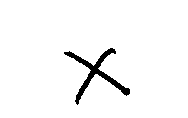
\includegraphics{bilder/eval_2.png}\\
        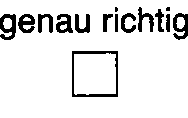
\includegraphics{bilder/eval_3.png}\\
        
\includegraphics{bilder/eval_4.png}\\
        
\includegraphics{bilder/eval_5.png}\\
    }
}

\noindent Neben dem \hyperref[kummerkasten]{Kummerkasten} hast Du gegen Ende des
Semesters mit der \emph{Evaluation} noch eine Möglichkeit, Deine Profs und
TutorInnen zu bewerten. Das läuft dabei so ab, dass jemand von der Fachschaft
(in der Physik) oder von der ZUV (in der Mathe) in die Vorlesung kommt, eine
kleine Einleitung gibt und dann einen Bogen austeilt, den Du dann ausfüllst. In
den Tutorien der Mathe übernehmen die Tutoren die Evaluation.  Das ganze dient
zweierlei Zwecken: Zum Einen werden besonders schlechte (oder gute) Vorlesungen
mit den Dozierenden nachbesprochen um das Lehrniveau zu steigern bzw. zu
halten. Zum Anderen können Dir die Ergebnisse auch helfen, die richtigen
Vorlesungen oder Übungsgruppen zu wählen. Wenn der/die DozentIn sein/ihr
Einverständniss zur Veröffentlichung gegeben hat, dann findest Du die
Ergebnisse der letzten Semester z.B. vor dem Fachschaftsraum (im
Infoständer links der Tür), sowie im \gls{KIP}, im Hörsaalgebäude der Physik
(\Gls{INF} 308) und am Philosophenweg, jeweils an Infobrettern.
